
%(BEGIN_QUESTION)
% Copyright 2009, Tony R. Kuphaldt, released under the Creative Commons Attribution License (v 1.0)
% This means you may do almost anything with this work of mine, so long as you give me proper credit

This room pressure control system maintains a slightly positive pressure in a precision electronic assembly room to prevent dust from entering from the outside, while always ensuring a rapid flow rate of air through the room.  It regulates pressure by modulating two dampers: one introducing air to the room (``forced draft'') and one venting air from the room (``induced draft'').  A pressure transmitter outputs 4 mA at 0 "W.C room pressure and 20 mA at 2 "W.C. room pressure:
 
$$\includegraphics[width=15.5cm]{i03785x01.eps}$$

Assuming reverse action in the controller, determine the proper split ranges of the two control valves:

% No blank lines allowed between lines of an \halign structure!
% I use comments (%) instead, so that TeX doesn't choke.

$$\vbox{\offinterlineskip
\halign{\strut
\vrule \quad\hfil # \ \hfil & 
\vrule \quad\hfil # \ \hfil \vrule \cr
\noalign{\hrule}
%
% First row
Forced draft damper position & Controller output signal \cr
%
\noalign{\hrule}
%
% Another row
Fully shut (0\%) & ??? mA \cr
%
\noalign{\hrule}
%
% Another row
Wide open (100\%) & ??? mA \cr
%
\noalign{\hrule}
} % End of \halign 
}$$ % End of \vbox

% No blank lines allowed between lines of an \halign structure!
% I use comments (%) instead, so that TeX doesn't choke.

$$\vbox{\offinterlineskip
\halign{\strut
\vrule \quad\hfil # \ \hfil & 
\vrule \quad\hfil # \ \hfil \vrule \cr
\noalign{\hrule}
%
% First row
Induced draft damper position & Controller output signal \cr
%
\noalign{\hrule}
%
% Another row
Fully shut (0\%) & ??? mA \cr
%
\noalign{\hrule}
%
% Another row
Wide open (100\%) & ??? mA \cr
%
\noalign{\hrule}
} % End of \halign 
}$$ % End of \vbox

\vskip 20pt \vbox{\hrule \hbox{\strut \vrule{} {\bf Suggestions for Socratic discussion} \vrule} \hrule}

\begin{itemize}
\item{} A good problem-solving technique to apply in cases where we need to determine the direction of a change is to consider {\it limiting cases}.  Instead of asking ourselves what would happen if the room air pressure changes slightly, we ask ourselves what would happen if the room air pressure changes {\it dramatically}.  Explain how this problem-solving technique applies to this particular system.
\item{} Can you think of a more energy-efficient way of regulating air pressure in this ``clean room'' than using dampers?
\item{} Identify how this control system could be augmented to provide {\it air flow rate} control in addition to room pressure control.
\item{} What is the purpose of having an induced draft (ID) fan at all, since eliminating it entirely would {\it guarantee} positive pressure in the room so long as the forced draft (FD) fan was running?
\item{} Determine the most likely fail-states of each damper, assuming we wish to default to a condition where the room remains as clean as possible.
\item{} What would happen if the 4-20 mA signal cable between the controller and valves failed open in this system?  Explain your answer in detail.
\item{} What would happen if the 4-20 mA signal cable between the controller and valves failed shorted in this system?  Explain your answer in detail.
\item{} What would happen if the 4-20 mA signal cable between the controller and transmitter failed open in this system?  Explain your answer in detail.
\item{} What would happen if the 4-20 mA signal cable between the controller and transmitter failed shorted in this system?  Explain your answer in detail.
\end{itemize}


\underbar{file i03785}
%(END_QUESTION)





%(BEGIN_ANSWER)

% No blank lines allowed between lines of an \halign structure!
% I use comments (%) instead, so that TeX doesn't choke.

$$\vbox{\offinterlineskip
\halign{\strut
\vrule \quad\hfil # \ \hfil & 
\vrule \quad\hfil # \ \hfil \vrule \cr
\noalign{\hrule}
%
% First row
Forced draft damper position & Controller output signal \cr
%
\noalign{\hrule}
%
% Another row
Fully shut (0\%) & 4 mA \cr
%
\noalign{\hrule}
%
% Another row
Wide open (100\%) & 20 mA \cr
%
\noalign{\hrule}
} % End of \halign 
}$$ % End of \vbox

% No blank lines allowed between lines of an \halign structure!
% I use comments (%) instead, so that TeX doesn't choke.

$$\vbox{\offinterlineskip
\halign{\strut
\vrule \quad\hfil # \ \hfil & 
\vrule \quad\hfil # \ \hfil \vrule \cr
\noalign{\hrule}
%
% First row
Induced draft damper position & Controller output signal \cr
%
\noalign{\hrule}
%
% Another row
Fully shut (0\%) & 20 mA \cr
%
\noalign{\hrule}
%
% Another row
Wide open (100\%) & 4 mA \cr
%
\noalign{\hrule}
} % End of \halign 
}$$ % End of \vbox


\vskip 10pt

Hint: I suggest a ``thought experiment'' whereby you imagine a process condition far from setpoint, and then you imagine what valve positions would be necessary to bring the process variable back to setpoint.

%(END_ANSWER)





%(BEGIN_NOTES)

What we need is this type of split-ranging (assuming reverse control action):

$$\includegraphics[width=15.5cm]{i03785x02.eps}$$


\vskip 20pt \vbox{\hrule \hbox{\strut \vrule{} {\bf Suggestions for Socratic discussion} \vrule} \hrule}

\begin{itemize}
\item{} How well would this system function if the split-ranging on the ID and FD dampers were {\it exclusive} rather than {\it complementary}?
\item{} How well would this system function if the split-ranging on the ID and FD dampers were {\it progressive} rather than {\it complementary}?
\end{itemize}

%INDEX% Final Control Elements, valve: split ranging
%INDEX% Process: clean room pressure control

%(END_NOTES)


